\documentclass{article}
\usepackage[utf8]{inputenc}

\usepackage{amsmath, amssymb, amsthm, amsfonts}
\usepackage{subcaption, enumerate}
\usepackage{bbold}
\usepackage{polynom}
\usepackage{xfrac}
\usepackage{graphicx}
\usepackage{mathtools}
\usepackage{enumitem}

\usepackage{tikz}

\theoremstyle{definition}
\newtheorem{proposition}{Proposition}
\newtheorem{definition}{Definition}
\newtheorem{example}{Example}[definition]
\newcommand{\dab}
{
	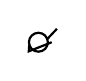
\begin{tikzpicture}[scale=0.04]
		% head
		\draw[thick] (0, 0) circle (3cm);

		% bent arm
		\draw[thick, rotate around={15 : (0, 0)}] (-3, 0) -- (-3.7, -2) -- (4.1, -1.1);

		% extended arm
		\draw[thick, rotate=20] (3, 0) -- (7, 2);
	\end{tikzpicture}
}
\newcommand{\st}{\text{ s.t. }}

\makeatletter
\renewcommand*\env@matrix[1][*\c@MaxMatrixCols c]{%
  \hskip -\arraycolsep
  \let\@ifnextchar\new@ifnextchar
  \array{#1}}
\makeatother

\usepackage{fullpage}

\title{Linear Transforms Day 6 \\ with Dr Nevard}
\author{Notes by Laura Gallo}
\date{October 5, 2020}

\begin{document}
\maketitle

\section{Matrix Terminology}
Given a linear transformation $T\in\mathcal{L}(V,W)$ and its corresponding matrix $A=\mathcal{M}(T)$, the following hold:

\begin{proposition}
	$T$ is invertible if and only if $A$ is nonsingular
\end{proposition}

\begin{definition}
	Given $T\in\mathcal{L}(V)$, where $V$ is an inner product space:
	$$\exists!T^\ast\in\mathcal{L}\st\forall v,w\in V,<Tv,w> = <v,T^\ast w>$$
	This unique $T^\ast$ is called the adjoint of $T$.
	If an orthonormal basis is chosen:
	\begin{equation*}
			\mathcal{M}(T^\ast)=\begin{cases}
				\text{transpose of $A$, $A^T$ ($b_{ij}=a_{ji}$)} & \text{if real} \\
				\text{conjugate transpose of $A$, $\overline{A^T}$ ($b_{ij}=\overline{a_{ji}}$)} & \text{if complex}
		\end{cases}
	\end{equation*}
\end{definition}

\begin{definition}
	If $T=T^\ast$, $T$ is self adjoint. Analogously, this means that
	\begin{equation*}
		A=\begin{cases}
			\text{$A^T$ is symmetric} & \text{if real} \\
			\text{$\overline{A^T}$ is Hermitian symmetric} & \text{if complex}
		\end{cases}
	\end{equation*}
\end{definition}
\begin{definition}
	If $T^{-1}=T^\ast$, then
	\begin{equation*}
		\begin{cases}
			AA^T=I \text{ and $A$ is orthogonal} & \text{if real} \\
			A\overline{A^T}=I \text{ and $A$ is unitary} & \text{if complex} \\
		\end{cases}
	\end{equation*}
\end{definition}
\end{document}
